\subsection{SFML}

Au début de notre projet, nous avions pensé à utiliser une bibliothèque graphique spécialisée dans la réalisation de jeu, SFML (\textit{Simple and Fast Multimedia Library}).\\

Cette bibliothèque nous aurait permis de réaliser facilement des animations et divers effets graphiques. 
Cependant, en utilisant SFML, des comportements inattendus ont été constatés, notamment au niveau de l'affichage des fenêtres SFML dans la QMdiArea de Qt. La QMdiArea est une zone dans laquelle des sous-fenêtres gérées par Qt peuvent être ouvertes. Parmi les problèmes présents, nous pouvions observer un problème de tremblement concernant les sous-fenêtres de carte, une trace laissée lors d'un défilement de la QMdiArea (voir figure \ref{fig:sfml_tracebug}), ainsi qu'une trace laissé par le passage d'une sous-fenêtre au dessus d'une autre (voir figure \ref{fig:sfml_movementbug}).

\begin{figure}[h!]
        \centering
        \begin{subfigure}[h!]{0.5\textwidth}
                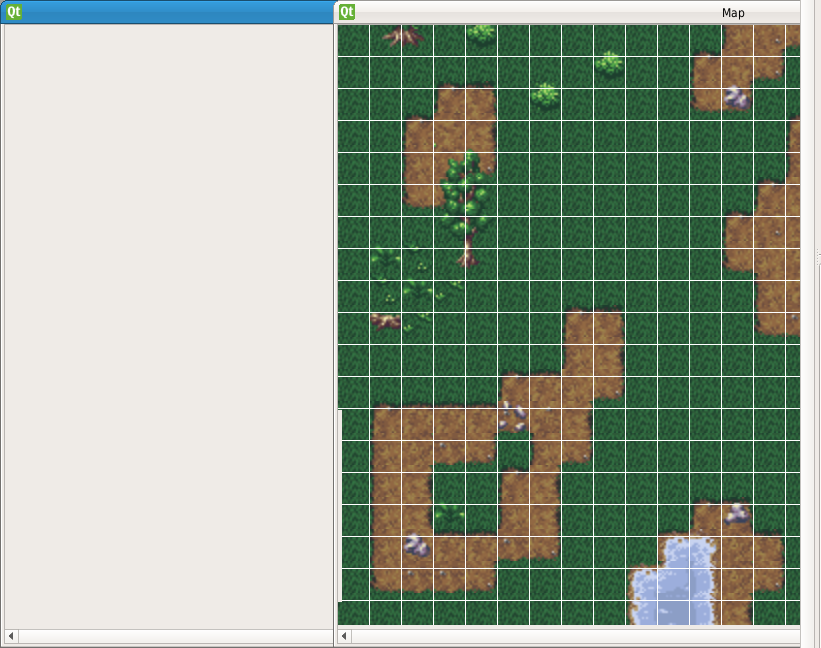
\includegraphics[width=\textwidth]{img/sfml_traceBug.png}
				\caption{Problème lors du défilement de la QMdiArea}
				\label{fig:sfml_tracebug}
        \end{subfigure}%
    	~
        \begin{subfigure}[h!]{0.5\textwidth}
                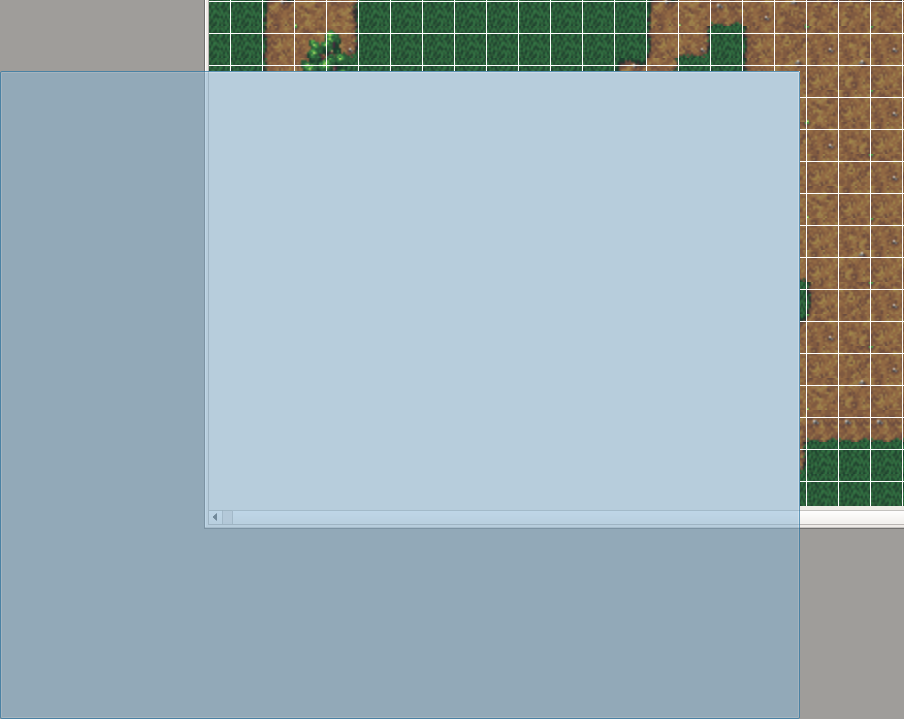
\includegraphics[width=\textwidth]{img/sfml_movementBug.png}
                \caption{Problème lors du déplacement d'une sous-fenêtre au dessus d'une autre}
				\label{fig:sfml_movementbug}
        \end{subfigure}
\end{figure}

Nous avons tout d'abord tenté de résoudre ces problèmes sans succès, puis de contourner les problèmes de différentes manières :
\begin{itemize}
	\item modifier le framerate des fenêtres SFML;
	\item cacher le contenu de la fenêtre pendant un déplacement et un redimensionnement;
	\item empêcher le défilement dans la QMdiArea.
\end{itemize}
 
Après avoir tenté d'inclure SFML dans Qt durant deux semaines, nous avons décidé de réaliser l'application exclusivement avec Qt. En effet, la carte était fonctionnelle, mais nous redoutions l'apparition de problèmes futurs. De plus, les comportements anormaux décrits plus haut ont été contournés plutôt que corrigés, ce qui nous dérangeait. Nous avons donc dû repenser entièrement le système de carte déjà réalisé avec SFML.